% =========================================================
% Stern--Brocot Tree (first few levels)
% =========================================================

\begin{figure}[h]
\centering
\begin{tikzpicture}[
  level distance=1.4cm,
  sibling distance=7.5cm,
  every node/.style={font=\small},
  edge from parent/.style={draw, -}
]

\node {$\frac{1}{1}$}
  child {
    node {$\frac{1}{2}$}
    child {
      node {$\frac{1}{3}$}
      child {
        node {$\frac{1}{4}$}
      }
      child {
        node {$\frac{2}{5}$}
      }
    }
    child {
      node {$\frac{2}{3}$}
      child {
        node {$\frac{3}{5}$}
      }
      child {
        node {$\frac{3}{4}$}
      }
    }
  }
  child {
    node {$\frac{2}{1}$}
    child {
      node {$\frac{3}{2}$}
      child {
        node {$\frac{4}{3}$}
      }
      child {
        node {$\frac{5}{3}$}
      }
    }
    child {
      node {$\frac{3}{1}$}
      child {
        node {$\frac{5}{2}$}
      }
      child {
        node {$\frac{4}{1}$}
      }
    }
  };

% Optional side labels for the sentinels
\node[left=2.8cm] at ([xshift=-2.8cm,yshift=0cm]current bounding box.west) {};

\end{tikzpicture}
\caption{The Stern--Brocot tree. Each child is obtained by taking mediants between neighboring fractions.}
\label{fig:stern-brocot-tree}
\end{figure}




% =========================================================
% Stern--Brocot Tree with sentinels
% =========================================================

\begin{figure}[h]
\centering
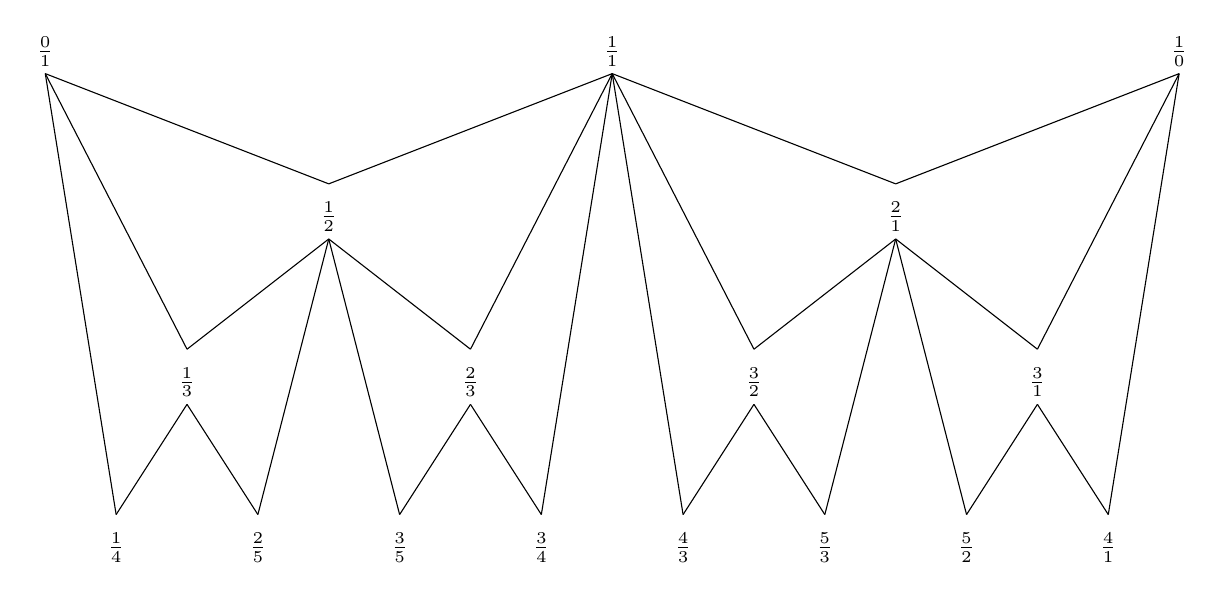
\begin{tikzpicture}[x=1.2cm,y=1.4cm, every node/.style={font=\small}]

% Top sentinels and root
\node at (-6,0) {$\frac{0}{1}$};
\node at ( 0,0) {$\frac{1}{1}$};
\node at ( 6,0) {$\frac{1}{0}$};

% Level 1
\node at (-3,-1.5) {$\frac{1}{2}$};
\node at ( 3,-1.5) {$\frac{2}{1}$};

% Level 2
\node at (-4.5,-3) {$\frac{1}{3}$};
\node at (-1.5,-3) {$\frac{2}{3}$};
\node at ( 1.5,-3) {$\frac{3}{2}$};
\node at ( 4.5,-3) {$\frac{3}{1}$};

% Level 3
\node at (-5.25,-4.5) {$\frac{1}{4}$};
\node at (-3.75,-4.5) {$\frac{2}{5}$};
\node at (-2.25,-4.5) {$\frac{3}{5}$};
\node at (-0.75,-4.5) {$\frac{3}{4}$};
\node at ( 0.75,-4.5) {$\frac{4}{3}$};
\node at ( 2.25,-4.5) {$\frac{5}{3}$};
\node at ( 3.75,-4.5) {$\frac{5}{2}$};
\node at ( 5.25,-4.5) {$\frac{4}{1}$};

% Edges from root to sentinels
\draw (-6,-0.2) -- (-3,-1.2);
\draw ( 0,-0.2) -- (-3,-1.2);
\draw ( 0,-0.2) -- ( 3,-1.2);
\draw ( 6,-0.2) -- ( 3,-1.2);

% Edges level 1 to level 2
\draw (-6,-0.2) -- (-4.5,-2.7);
\draw (-3,-1.7) -- (-4.5,-2.7);

\draw (-3,-1.7) -- (-1.5,-2.7);
\draw ( 0,-0.2) -- (-1.5,-2.7);

\draw ( 0,-0.2) -- ( 1.5,-2.7);
\draw ( 3,-1.7) -- ( 1.5,-2.7);

\draw ( 3,-1.7) -- ( 4.5,-2.7);
\draw ( 6,-0.2) -- ( 4.5,-2.7);

% Edges level 2 to level 3
\draw (-6,-0.2) -- (-5.25,-4.2);
\draw (-4.5,-3.2) -- (-5.25,-4.2);

\draw (-4.5,-3.2) -- (-3.75,-4.2);
\draw (-3,-1.7)   -- (-3.75,-4.2);

\draw (-3,-1.7)   -- (-2.25,-4.2);
\draw (-1.5,-3.2) -- (-2.25,-4.2);

\draw (-1.5,-3.2) -- (-0.75,-4.2);
\draw ( 0,-0.2)   -- (-0.75,-4.2);

\draw ( 0,-0.2)   -- ( 0.75,-4.2);
\draw ( 1.5,-3.2) -- ( 0.75,-4.2);

\draw ( 1.5,-3.2) -- ( 2.25,-4.2);
\draw ( 3,-1.7)   -- ( 2.25,-4.2);

\draw ( 3,-1.7)   -- ( 3.75,-4.2);
\draw ( 4.5,-3.2) -- ( 3.75,-4.2);

\draw ( 4.5,-3.2) -- ( 5.25,-4.2);
\draw ( 6,-0.2)   -- ( 5.25,-4.2);

\end{tikzpicture}
\caption{The Stern--Brocot tree with sentinel fractions $\frac01$ and $\frac10$. Each new fraction is the mediant of its two parent bounds.}
\label{fig:stern-brocot-sentinels}
\end{figure}




\begin{remark}[How the Stern--Brocot tree is generated]
Start with the two bounding fractions
\[
\frac01
\quad\text{and}\quad
\frac10.
\]
Their mediant is
\[
\frac{0+1}{1+0} = \frac11.
\]
Then insert mediants recursively between neighboring fractions. For example,
\[
\frac01,\ \frac11,\ \frac10
\]
produces
\[
\frac12 \text{ between } \frac01 \text{ and } \frac11,
\qquad
\frac21 \text{ between } \frac11 \text{ and } \frac10.
\]
Repeating this process generates the Stern--Brocot tree.

Every positive rational number appears exactly once in reduced form in this tree.
\end{remark}


\begin{remark}[Why the Stern--Brocot tree matters]
The Stern--Brocot tree organizes the positive rational numbers by repeated mediants.
It provides a constructive way to search for rational approximations and makes the density
of $\mathbb{Q}$ visually transparent: between any two neighboring fractions, another rational
can always be inserted by taking the mediant.
\end{remark}



